\documentclass[a4paper]{article}
\usepackage{graphicx}
\usepackage{epstopdf}
\usepackage{mcode}
\usepackage{style}
\usepackage{float}
\title{Laboration i Komponentfysik\\ Optoelektronik}

\author{Alexander Najafi \\ Linus Hellman}

\date{2014-04-13}

\begin{document}

\maketitle
\thispagestyle{empty}
\newpage

\tableofcontents
\newpage

\section{Inledning och bakgrund}

Denna lab är utformad för att ge en större förståelse för halvledarkomponenter och dess samverkan med ljus, både emission (ljusluminicens) samt absorption kommer undersökas. Detta har ett extremt stort användningsområde tillexempel i kameror, där ljus ska översättas till digital data. Under labben kommer det kontrolleras om det stämmer att den våglängd som stämmer överens med bandgapsenerginkommer att lysa med störst intensitet. Vidare kommer också absorptionskurvan att studeras. Teorin säger att fotodioden kommer börja absorbera fotoner i rymdladdningsområdet först då fotonerna har en våglängd som ger en energi som är lika med eller större än bandgapsenergin enligt $\lambda = hc/E_{fot}$, men då rymdladdningsområdet ligger en bit under ytan kommer absorptionskonstanten att öka i takt med fotonenergin och det leder till att absorptionen kommer minska igen enligt följande formel.

\begin{equation}
  \Phi(x) =\Phi_0e^{-\alpha x}
\end{equation}

Diodens uppbyggnad kommer även studeras då en egen diod kommer tillverkas och analyseras. Denna kommer konstrueras med hjälp av en platta av Galliumfosfid som kommer legeras med dels tenn dels zinklegerat guld. Detta kommer att n-,p-dopa GaP-biten tillräckligt för att den ska få en diods egenskaper. 

Vidare kommer en analys göras på en solcell för att undersöka vid vilken belastningsresistans denna uppnår sin maximala effekt. Belysning av en diod kommer att leda till en ström genom dioden. Men om ingen belastningsresistans finns kommer det inte ligga någon spänning över dioden alltså ingen effekt. Om det istället ligger oändligt mycet belastning över dioden kommer det inte att gå någon ström, alltså ingen effekt. Det som måste göras är att hitta den punkt i ström/spänningkurvan som ger den största arean ($U*I=effekten$).
\section{Utförande}
\subsection{Emission och absorption av lysdioder}
För att kunna mäta absorption och emission av lysdioder användes uppställningen som synes i figur \ref{eauppstln}. Först placerades en diod som ljuskälla i uppställningen (ljus in i figur \ref{eauppstln}) och en fotodetektor efter utgångsspalten. Prismat i uppställningen spred ut ljuset från dioden i olika våglängder. Genom att vrida på prismat kunde därför ljus med olika våglängd riktas mot detektorn och undersökas. I datorn fanns ett labviewprogram som styrde prismats vinkel, programmet tog även emot data från detektorn. Programmet användes för att svepa prismat så att det snliga spektrat kunde undersökas. Samtidigt som prismat rörde sig samplades data från detektorn för att kunna skapa ett diagram som visade intensiteten som en funktion av våglängderna i ljuset från dioden. 

För att mäta absorptionen placerades istället en lampa som ingångsljus, på utgången i uppställningen placerades dioden. Samma programma som tidigare användes för att svepa prismat över olika våglängder. ??Strömmen(eller spänningen)??? mättes över dioden och användes för att skapa ett diagram som visade hur absorptionen berodde på väglängden i det infallande ljuset. 

\subsection{Tillverkning av GaP-diod}
För att tillverka en GaP-diod användes en liten bit GaP, en tennkula och en zinklegerad guldtråd. Tråden och tennkulan placerades på GaP-plattan som i sin tur placerades på ett tantalbleck. Blecket kunde värmas upp kraftigt genom att låta en stor ström gå genom det. När strömmen och temperaturen ökade smälte tennkulan och guldtråden. När dessa smält minskades strömmen snabbt så att tennkulan inte hann oxideras.

När dioden var tillverkad undersöktes dess IV-karakteristik genom att mäta strömmen genom den när spänningen över den ändrades. Detta gjordes med hjälp av ett oscilloskop och en tongenerator. 

\subsection{Solcellen}
Solcellen kopplades in till en ampermeter och en voltmeter så att spänningen över och strömmen genom den kunde mätas. En lampa med konstant ljus placerades ca 20 cm från solcellen. Genom att variera lasten på solcellen kunde spänningen och strömmen för den mätas. Datan från detta plottades upp i ett IV-diagram.

\newpage
\section{Resultat}
\subsection{Emission och absorption av lysdioder}
Undersökningarna av emission och absorption av lysdioden samanfattas av figur \ref{emabs}. Se bilaga för matlabkod.
\begin{figure}[H]
        \centering
        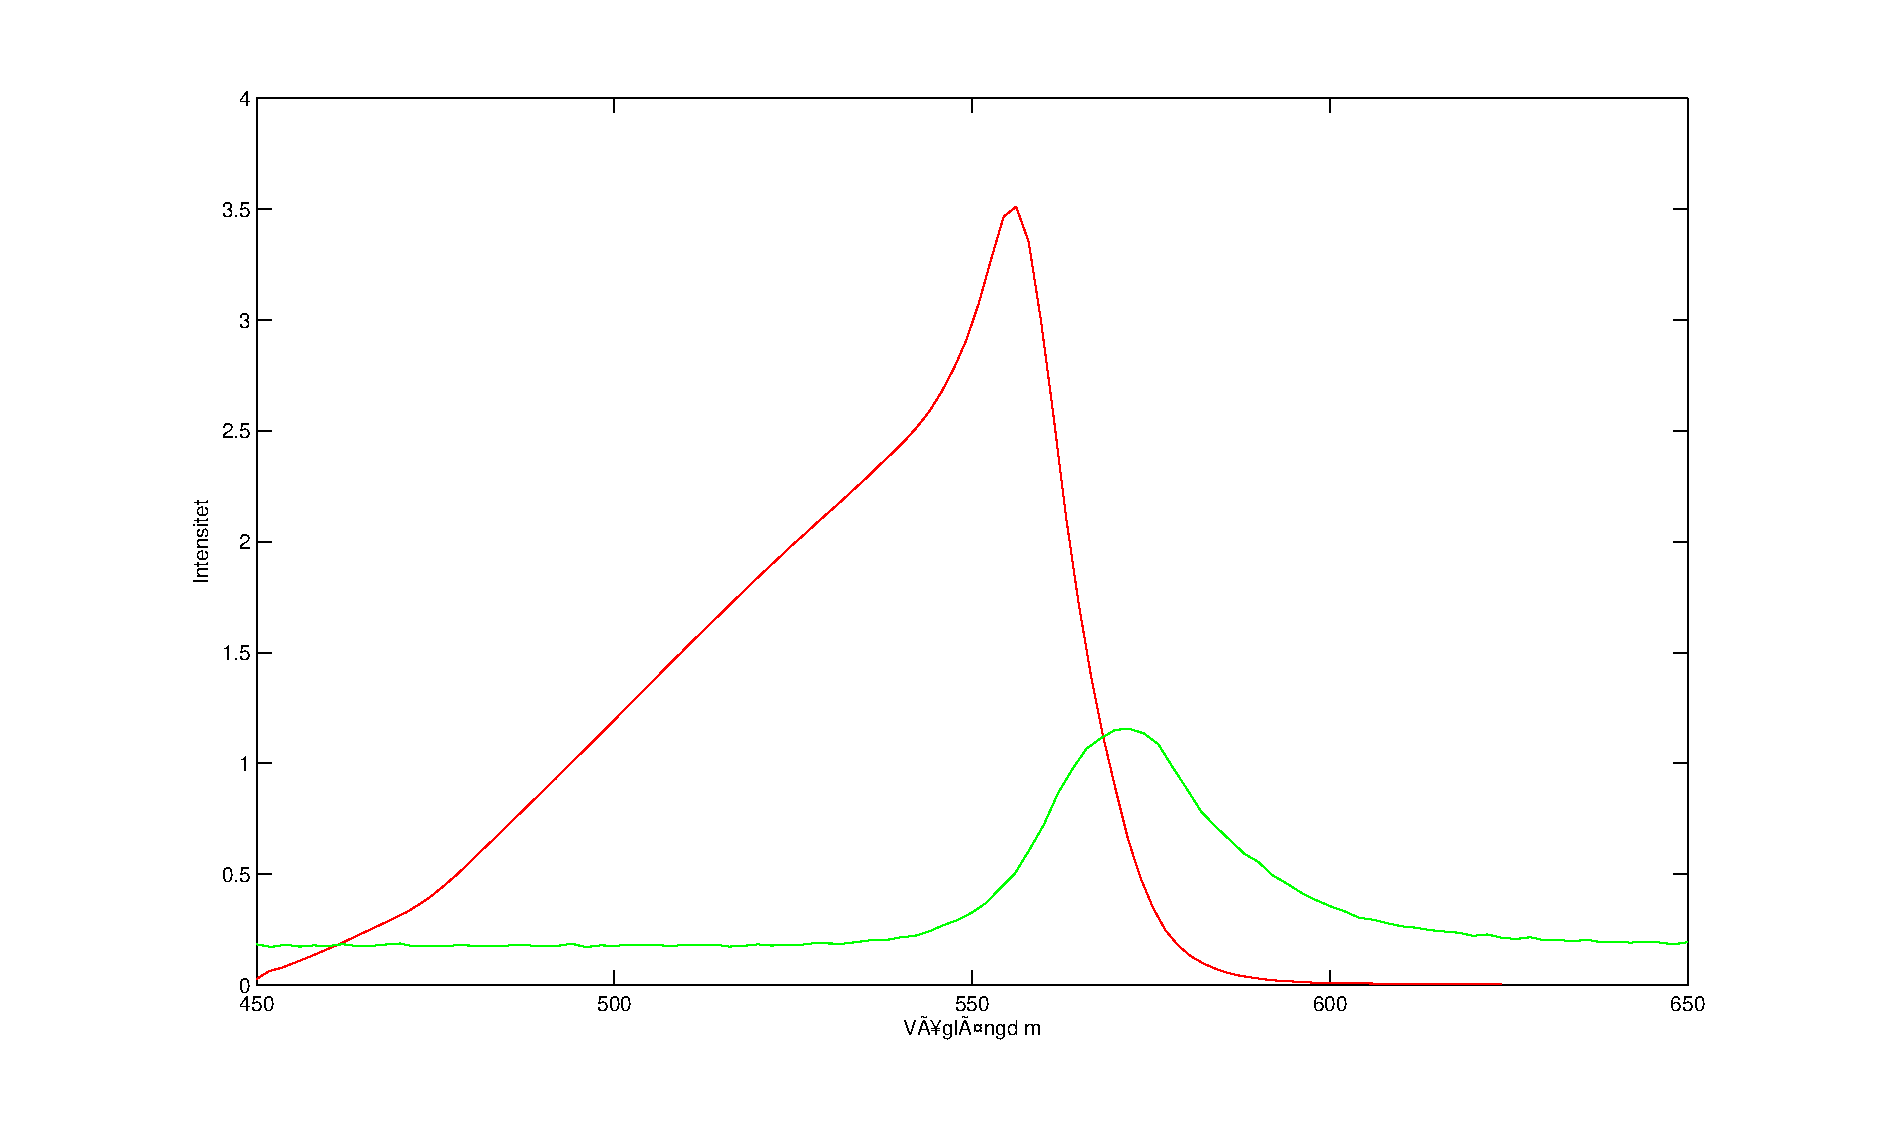
\includegraphics[scale=.4]{emabs.eps}
        \caption{Den gröna grafen visar emissionen och den röda visar absorptionen}
        \label{emabs}
\end{figure}

\subsection{Dioden}
Dioden som tillverkades hade en framspänning på 0.6V och en backspänning på 3.4V. I figur \ref{diodiv} synes I-V-kurvan som togs fram på labben med oscilloskopet.
\begin{figure}[H]
	\centering
	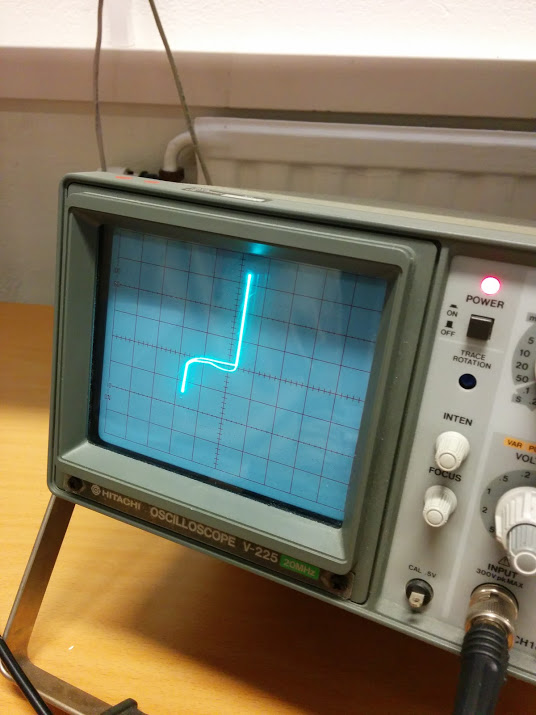
\includegraphics[scale=.4]{diod.jpg}
	\caption{I-V-kurva som syns på oscilloskopet}
	\label{diodiv}
\end{figure}
\subsection{Solcellen}
I-V-kurvan i figur \ref{solcelliv} togs fram för solcellen. För matlab-kod och data se bilaga.
\begin{figure}[H]
	\centering
	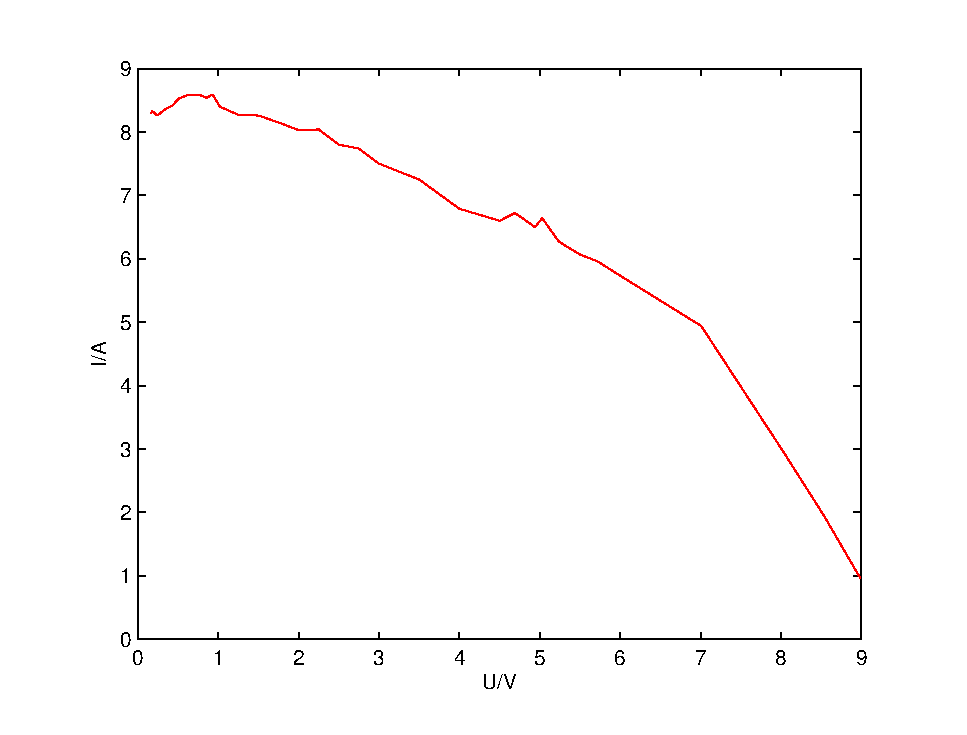
\includegraphics[scale=.7]{solcell.eps}
	\caption{I-V-kurva för solcellen}
	\label{solcelliv}
\end{figure}

\section{Analys och bearbetning av experimentell data}
\subsection{Emission och absorption av lysdioder}
Som synes i figur \ref{emabs} är absorptionen som högst kring en viss våglängd (kring 575nm) och väldigt nära 0nm för övrigt. Denna våglängd beror på bandgapet för dioden. Förhållandet mellan bandgapet och våglängden är $E = \frac{hc}{\lambda}$

En diod som absorberar ljus kommer absorbera alla fotoner med en energi större än bandgapet. Detta syns tydligt i figur \ref{emabs} på den röda kurvan. En foton med kortare våglängd har en större energi. Det syns en mycket tydlig brytpunkt där energin i fotonerna inte längre räcker till där intensiteten i absorptionen blir mycket liten och går mot 0. 

\subsection{Dioden}
Den egentillverkade dioden lyste med en våglängd kring 600nm vilket upskattades genom att använda en färgkarta och se vilken färg den lyste med. Detta kan jämföras med den teoretiskt korrekta våglängden som fås ur att veta bandgapet för galiumfosfid som är $2,26eV = 3,62*10^-19J$. Då vi vet att $E = \frac{hc}{\lambda}$ måste $\lambda = \frac{hc}{E}$ vilket ger den teoretiska våglängden

\begin{equation}
	\lambda = \frac{hc}{E} = \frac{6.626*10^{-34} * 3.0*10^8}{3,62*10^-19} = 549,11 nm.
\end{equation}

vilket är nära det gissade värdet. Resultatet för framspänningen och backspänningen på den tillverkade dioden stämmer också bra överens med teorin.

\subsection{Solcellen}

\section{Sammanfattning och slutsatser}
Under labben undersöktes bland annat diodens sammverkan med ljus. Då en diod används som emitter syntes det mycket tydligt att teorin stämde. Det emiterade ljuset når sin maxintensitet precis då våglängden stämmer överens med bandgapsenergin, detta syns på fig???. Även då dioden används som detektor kan man se att teorierna verkar stämma. Man ser en tydlig stegring av kurvan då den passerar bandgapsenergin och senare en sänkning i takt med att absorptionskonstanten ökar. Möjliga felkällor till detta moment skulle kunna innefatta att ljus utifrån läcker in och stör experimentet, men överlag märks det av marginellt lite. 

\newpage
\appendix
\section{Matlabkod}
\subsection{Emission och absorrption av dioder}
\lstinputlisting{absem.m}
\subsection{Solcellen}
\lstinputlisting{solcell.m}

\newpage
\section{Förberedelseuppgifter}
\begin{figure}[H]
\centering
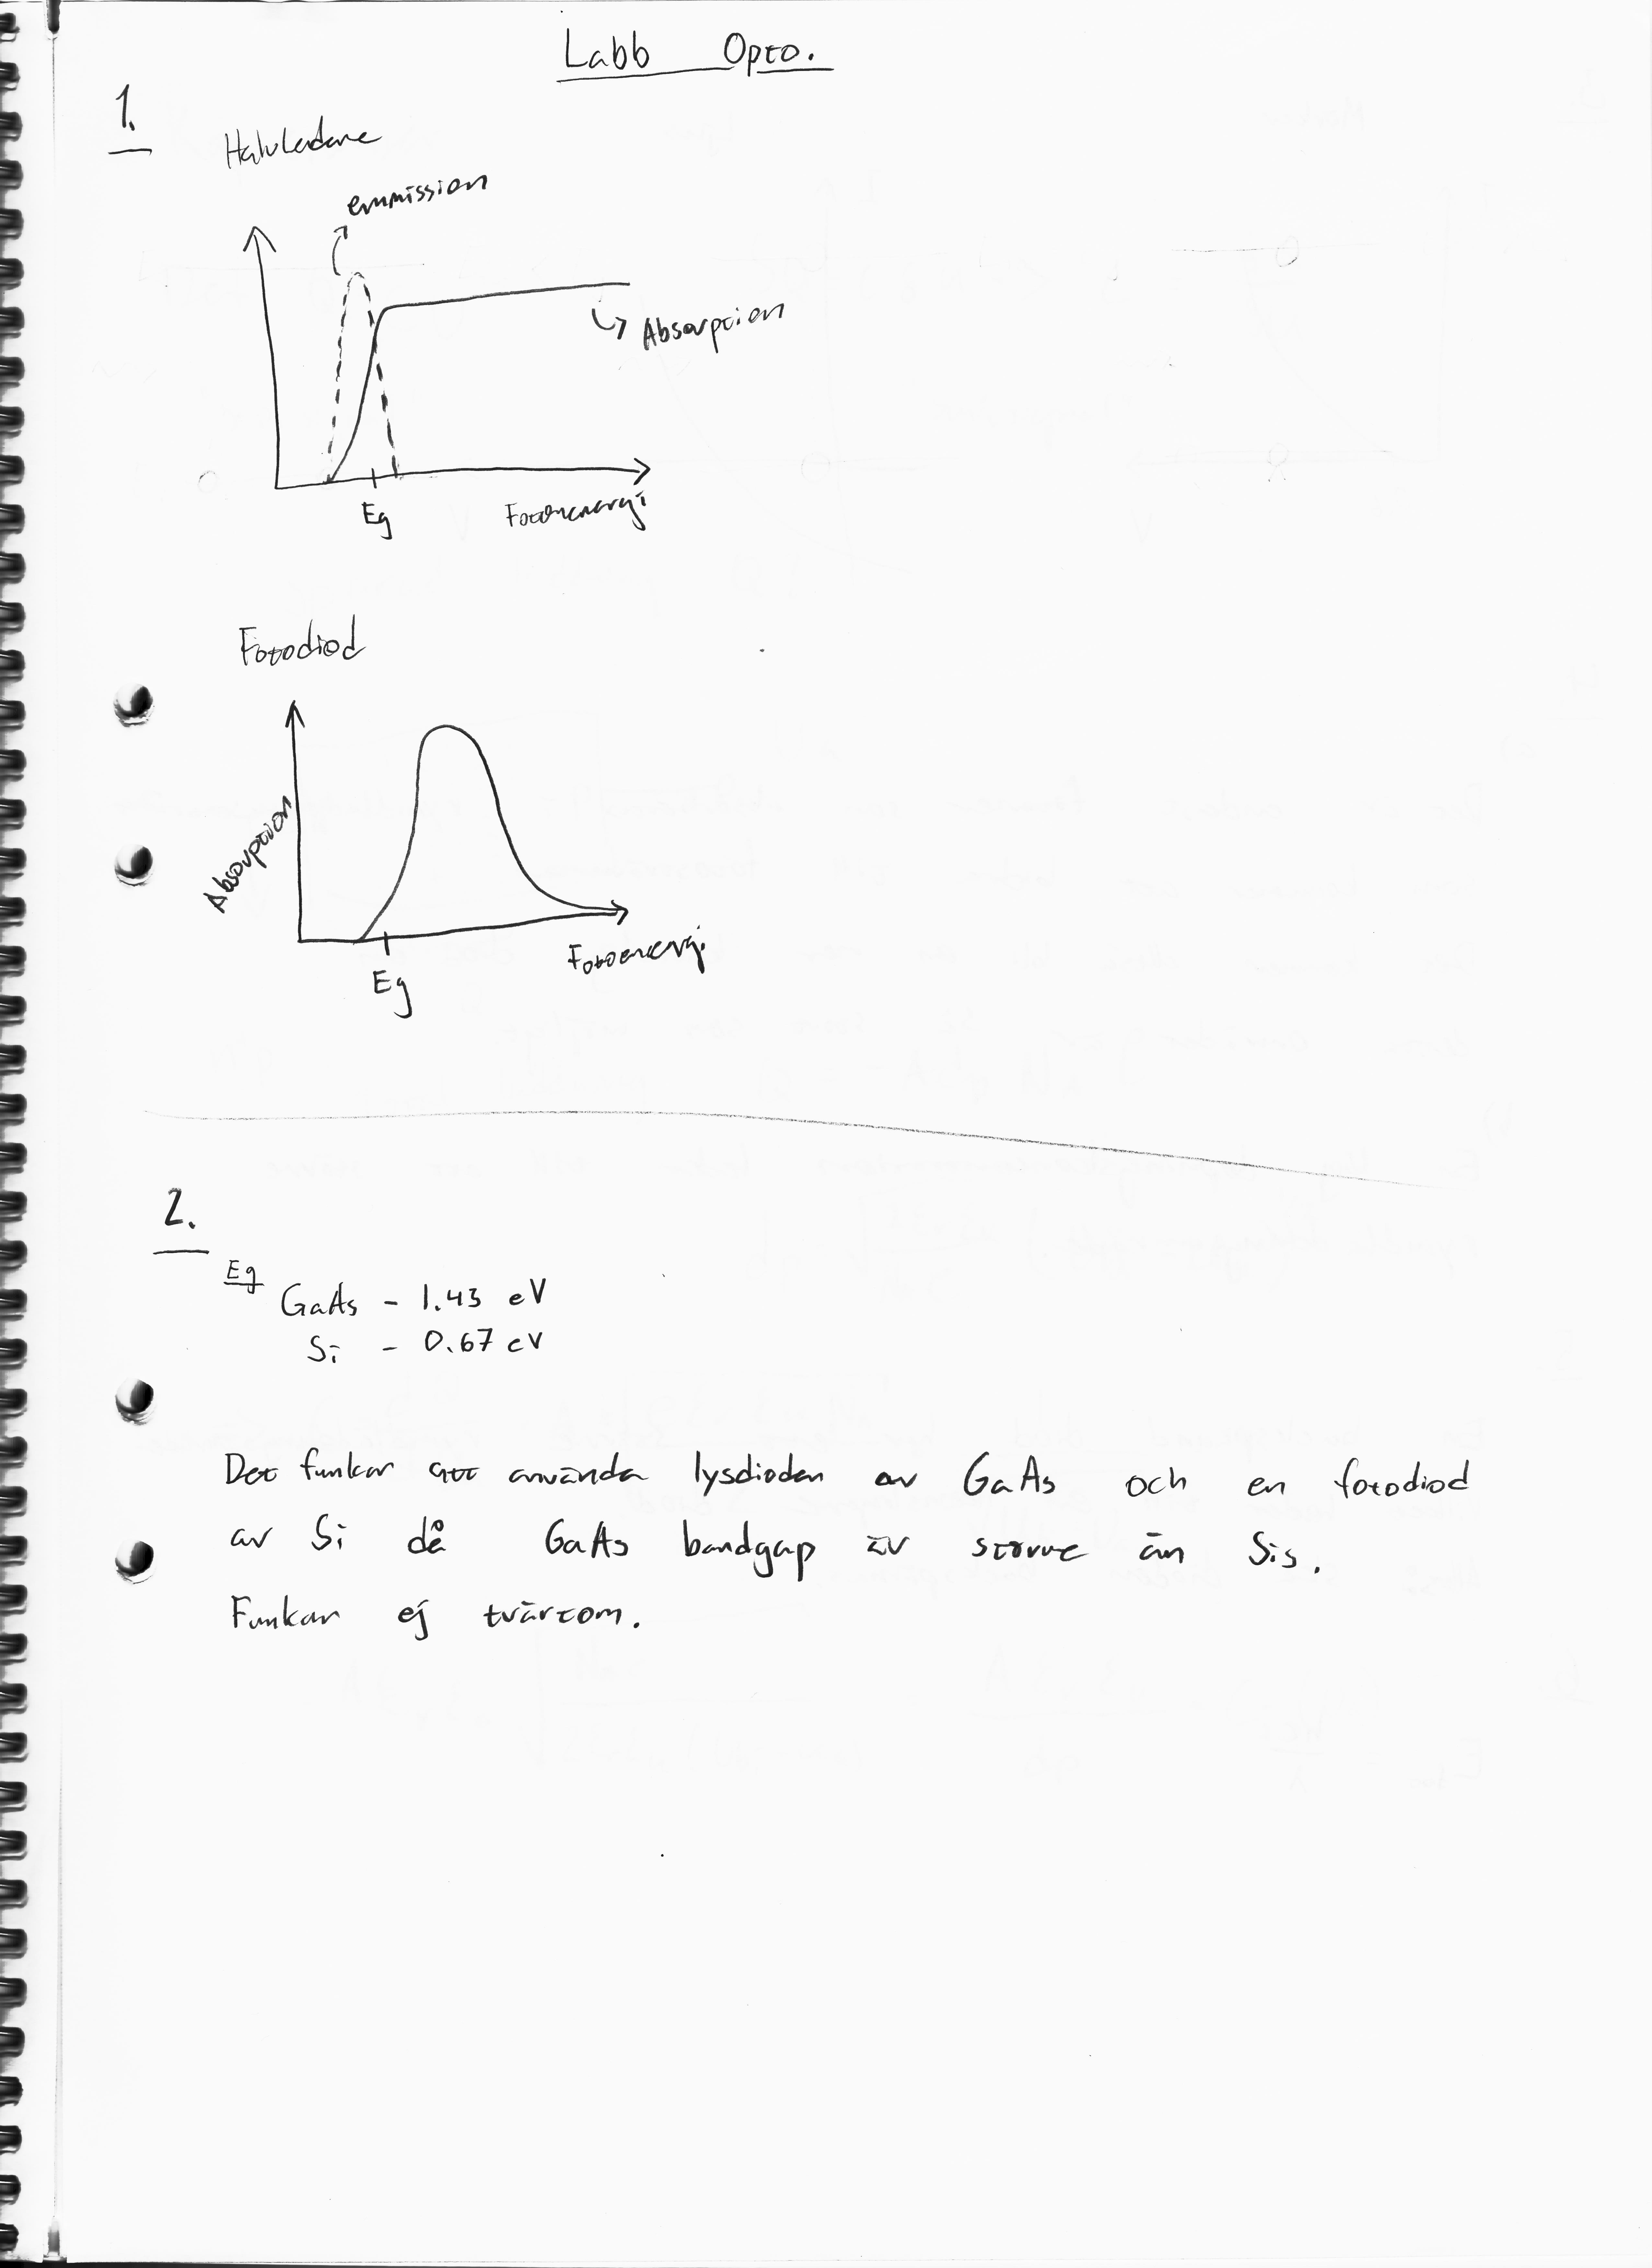
\includegraphics[scale=.7]{frb1.jpeg}
\end{figure}
\newpage
\begin{figure}[H]
\centering
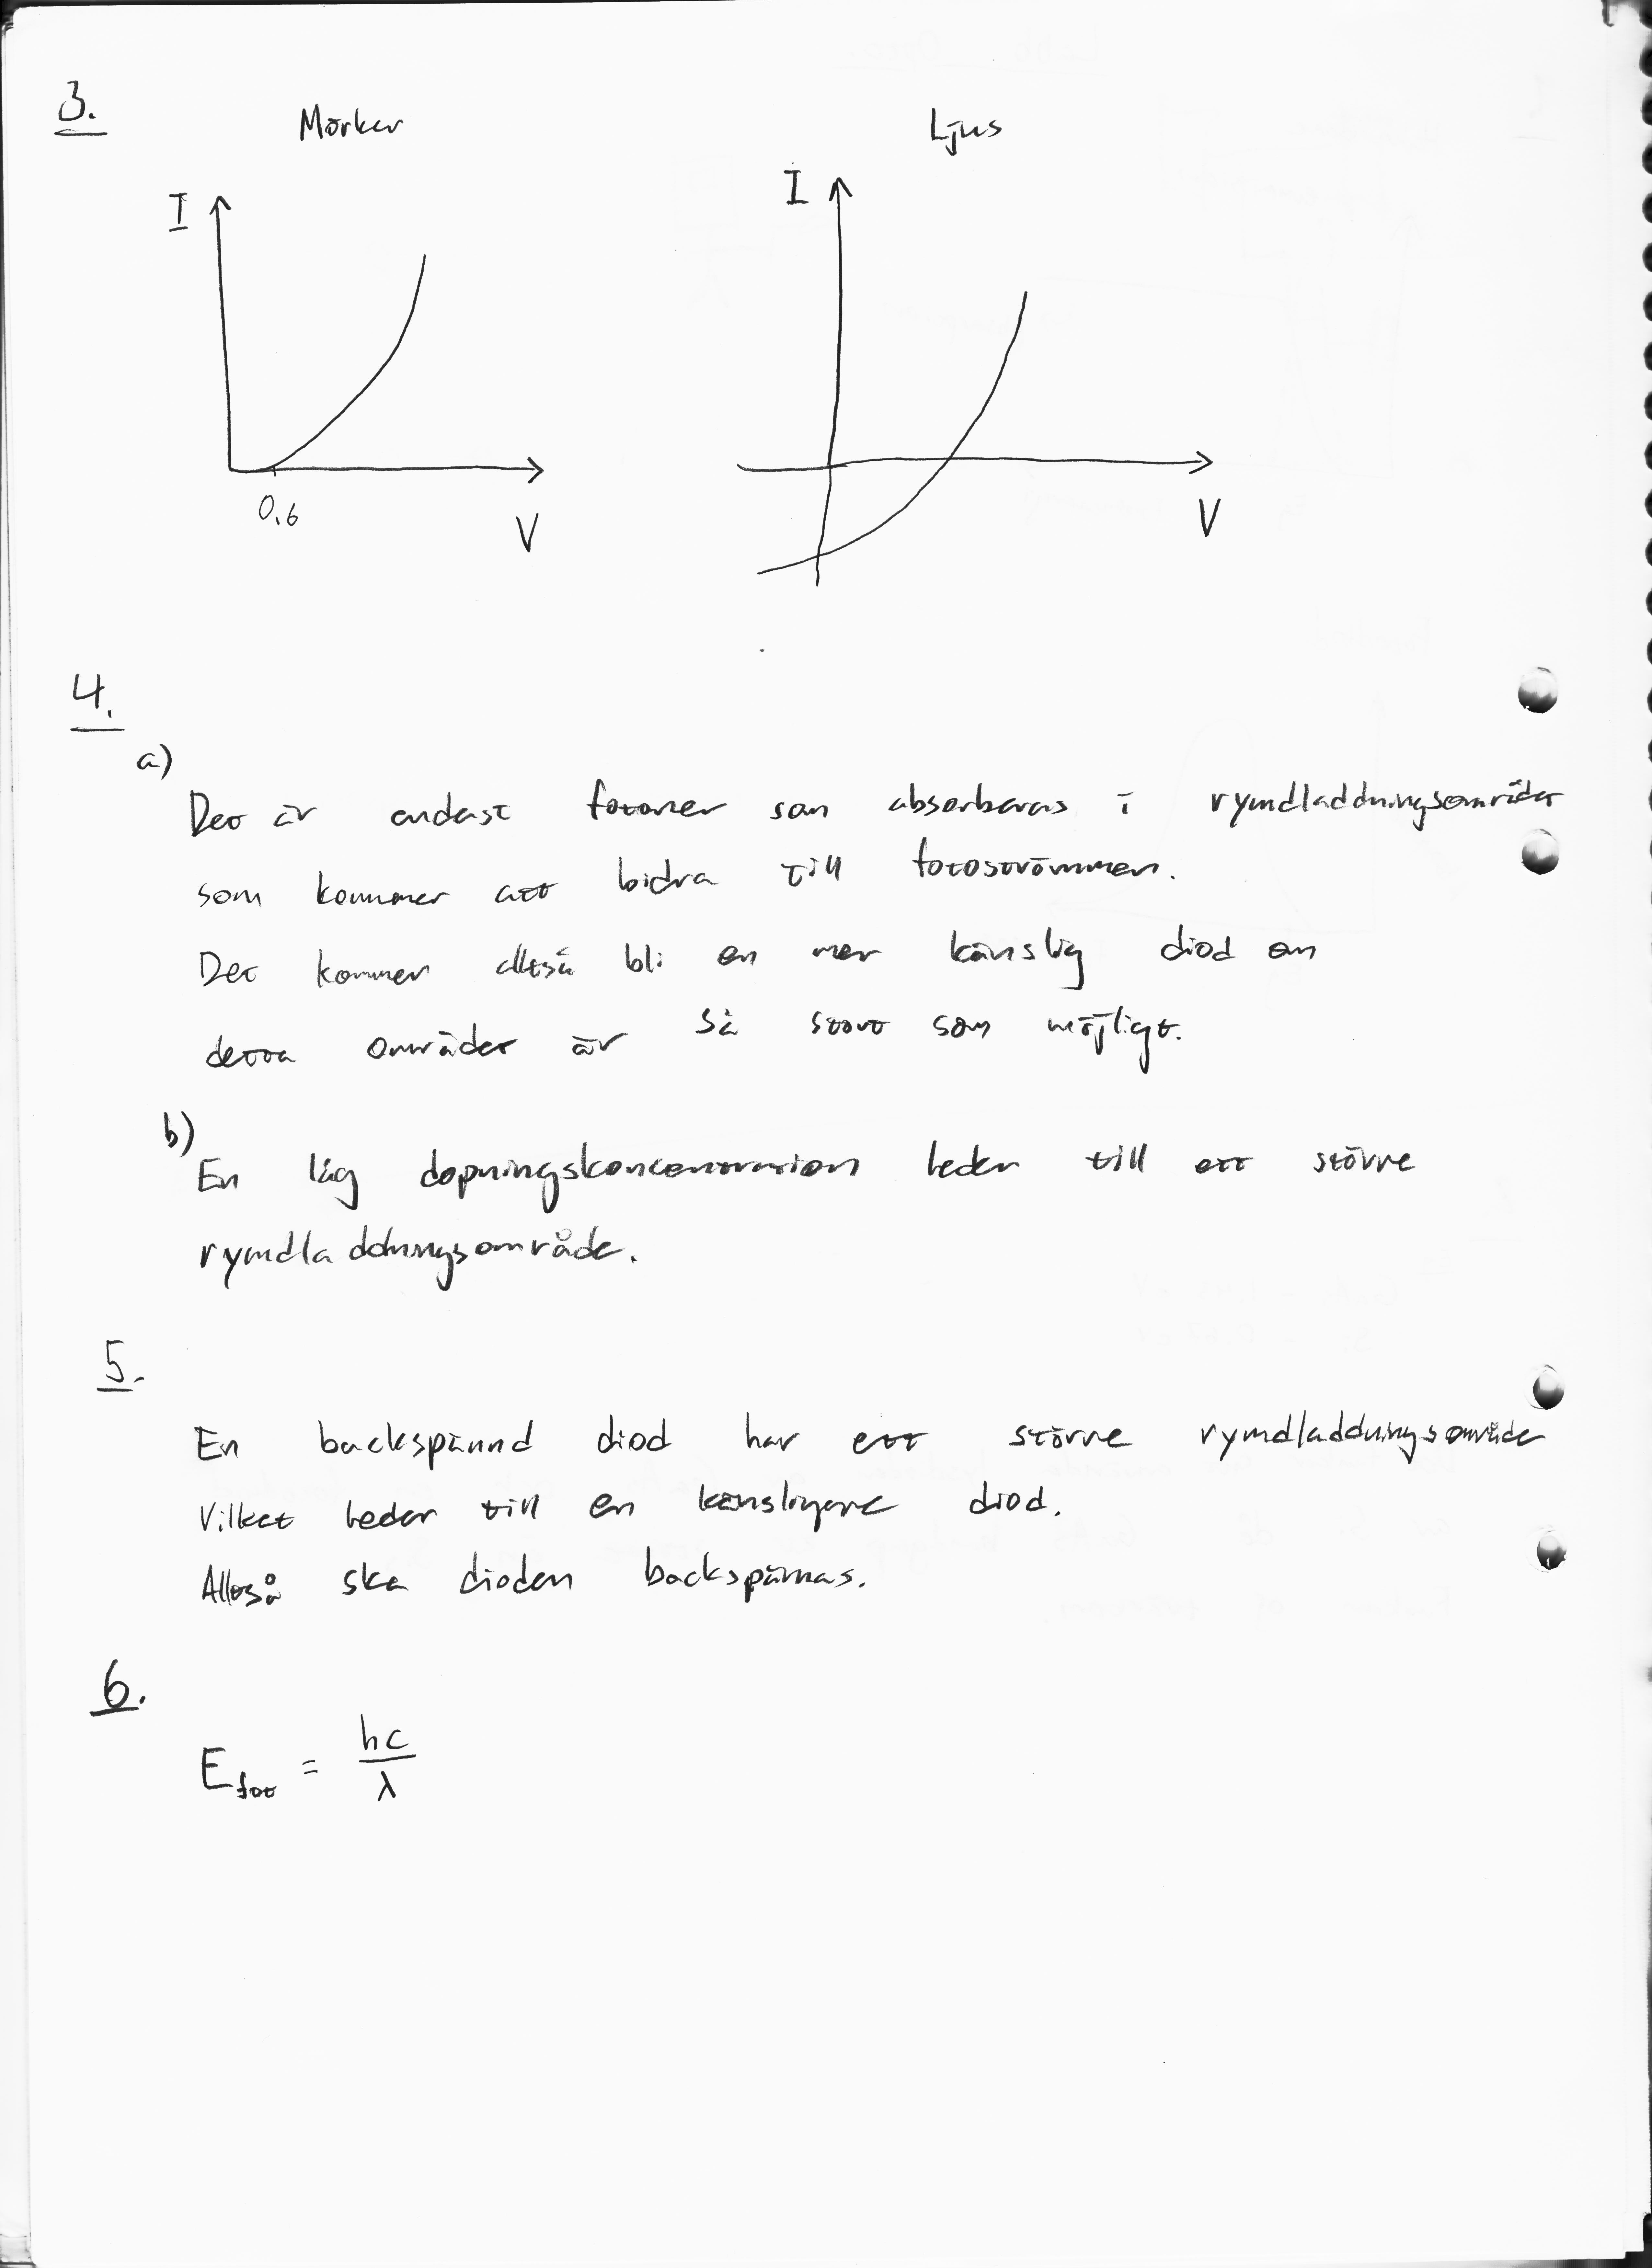
\includegraphics[scale=.7]{frb2.jpeg}
\end{figure}

\end{document}
